\section{Data models and formats}

This section gives an overview of the status and plans for the gamma-ray data model and formats. As mentioned before, this effort was only started very recently and none of the formats should be considered stable. The next two sections will describe the effort to define an event data model and format (DL3), and higher-level formats for images, spectra and lightcurves (DL4) (i.e. content split as already illustrated in Figure~\ref{fig:purpose})

In the data specification document we have created a "general" section that gives precise definitions of common quantities, such as precise definitions of time scales as well as coordinates systems. One example is a precise definition of \texttt{AZIMUTH} and \texttt{ALTITUDE}. We define \texttt{AZIMUTH} to be oriented east of north, and \texttt{ALTITUDE} to be relative to the zenith direction (not the horizon plane or a reference earth ellipsoid) and without applying a refraction correction.

There are some general questions we are discussing about where to be specific or flexible in our format specifications. One example is whether our data format specifications should be tied to FITS (and e.g. say the data type of a column is \texttt{1E}, which is the data type code for 32-bit float in FITS), or whether it would be better to only say that the data type is "float", implicitly allowing the storage of this column as 32-bit or 64-bit float, and being able to store the data e.g. in text ECSV files in addition to binary FITS files. Another contentious point is whether physical units should be fixed (e.g. "MeV" or "TeV"), or whether the units should be flexible and only serialization formats that support declaration of units (such as FITS or VOTABLE or ECSV) should be supported and science tools are expected to process the unit information correctly.

\subsection{Data level 3 (DL3) specifications}

DL3 format should describe all data released to the end users for analysis with science tools as , EVENT, IRF and TECH (technical data not directly attached to the object observed). Figure~\ref{fig:iact-dl3} illustrates some of the DL3 data content. Prototyping by existing IACTs (H.E.S.S., MAGIC, VERITAS and science tools (Gammapy, Ctools) is a major activity. 

\begin{figure}[tb]
\centerline{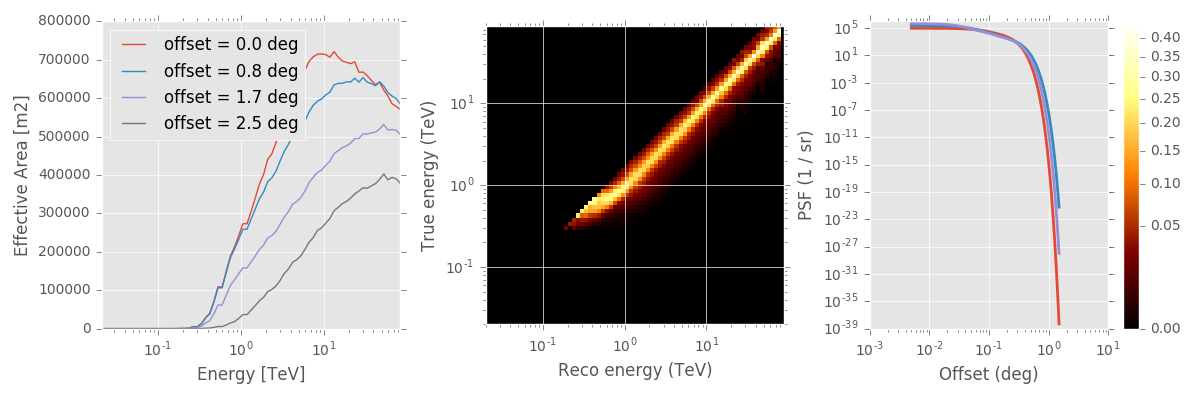
\includegraphics[width=0.9\textwidth]{figures/iact-dl3}}
\caption{
Illustration of major components of IACT ("imaging atmospheric Cherenkov telescope", here a H.E.S.S. 1 Crab nebula observation) DL3 ("data level 3") data. The \texttt{EVENTS} are stored as a table with the most important parameters shown. To derive spectra and morphology measurements of astrophysical sources, IRFs ("instrument response functions") are used: the effective area (\texttt{AEFF}), energy dispersion (\texttt{EDISP}) and point spread function (\texttt{PSF}). Sometimes background (\texttt{BKG}) models are also created and released as part of a DL3 data release, and can be treated like an IRF, and sometimes deriving background models is left to the science tools. Note that this picture is not complete, see the "IACT DL3" section.
}
\label{fig:iact-dl3}
\end{figure}

Many points are still under discussion/consideration:

\begin{itemize}
\item{}Observations modes, time intervals
\item{}How to link EVENT and IRF
\item{}Pointing and live time information
\item{}IRF axis and validity ranges
\item{}FoV coordinates
\end{itemize}

\subsection{Data level 4 \& 5 specifications}

A format is developed to store spectral analysis results for exchange and publication, not only "flux points" and "upper limits", but also the full likelihood profiles (see examples in Figure~\ref{fig:dl4-examples}).

\begin{figure}[tb]
\centerline{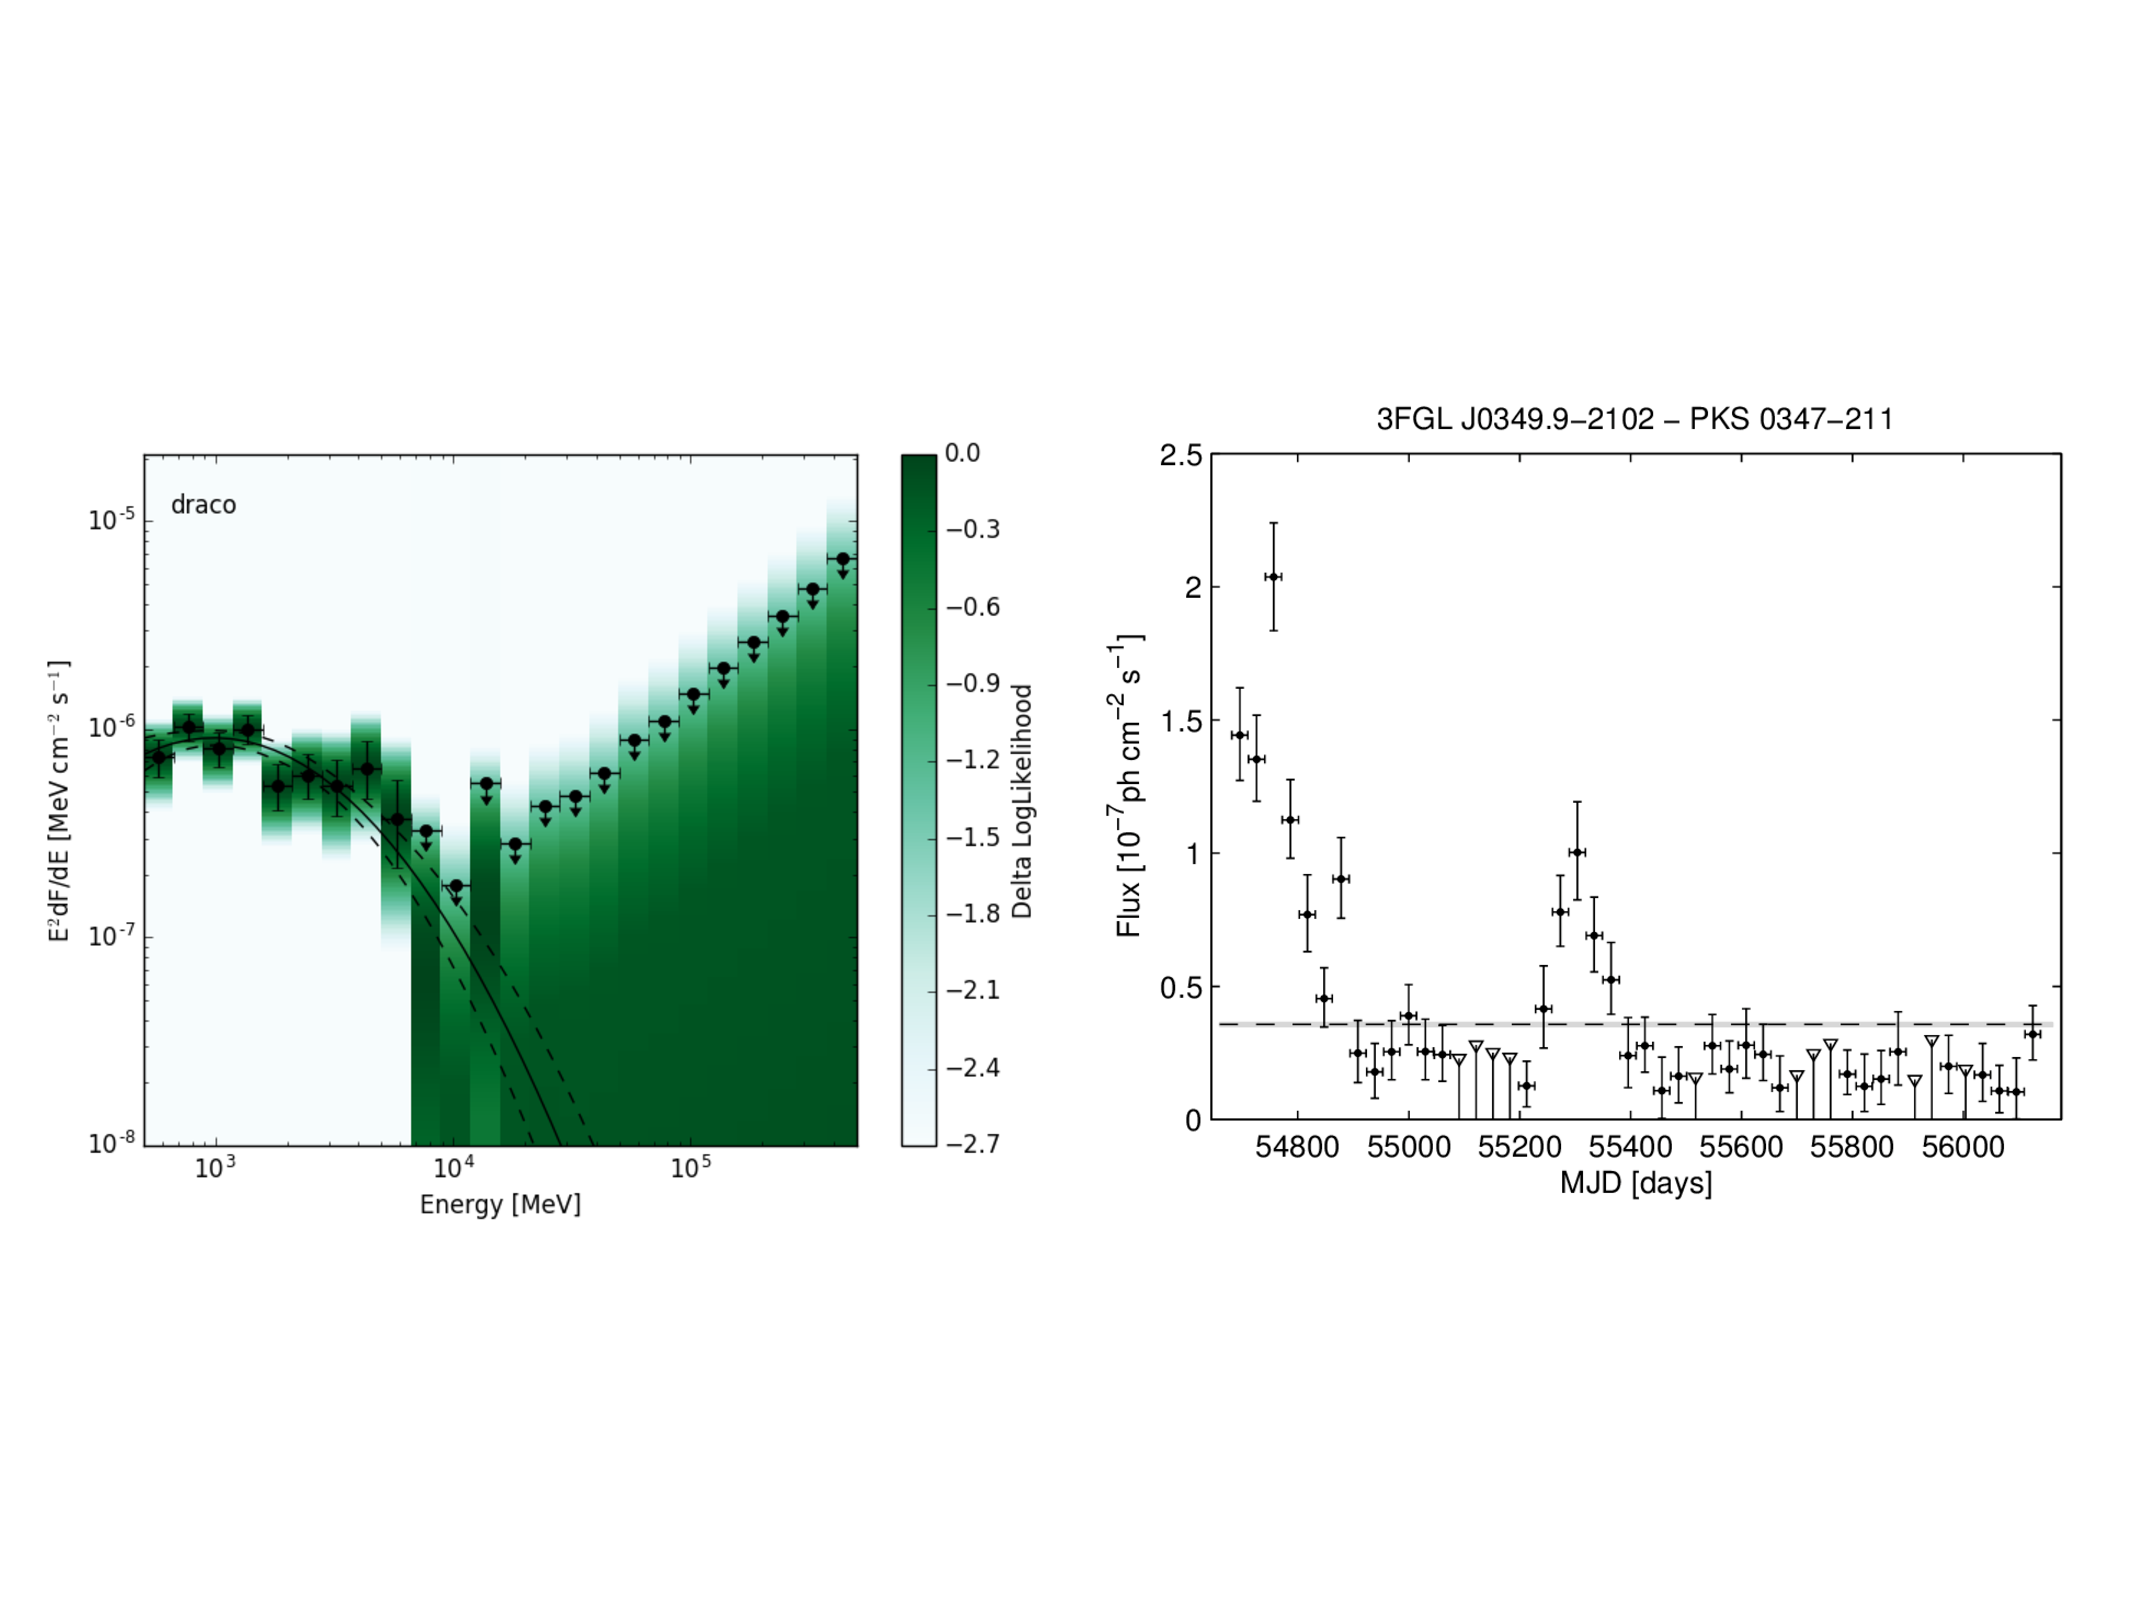
\includegraphics[width=\textwidth]{figures/dl4-examples}}
\caption{
Gamma-ray "data level 4" examples. \emph{Left:} spectral energy distribution (SED) likelihood profiles (green), with flux points and upper limits as well
as a best-model fit overplotted. \emph{Right:} Lightcurve of 3FGL~J0349.9-2102 from the third Fermi-LAT catalog.
}
\label{fig:dl4-examples}
\end{figure}

It was first developed in Fermipy\footnote{\url{https://github.com/fermipy/fermipy}} and used for Fermi-LAT (ref). It is now being adopted by ground-based high energy astronomy. Likelihood profiles are important information when those data are to be used in global spectral energy distribution (SED) of a source. 

Description of light curves is another topic open for discussion. 
